\documentclass{../homework}
\usepackage{ dsfont }

\name{Timothy Devon Morris}
\course{Me En 537}
\term{Fall 2018}
\hwnum{2}

\begin{document}

\begin{problem}[Corke Chap 2]
\end{problem}

\begin{solution}
  \begin{parts}
    \part 12

    Using the robotic toolbox with default options, I got
    \[
      R=
      \begin{bmatrix}
        c_{\theta}c_{\psi} & s_{\phi}s_{\theta}c_{\psi} - c_{\phi}s_{\psi} & c_{\phi}s_{\theta}c_{\psi} + s_{\phi}s_{\psi} \\
        c_{\theta}s_{\psi} & s_{\phi}s_{\theta}s_{\psi} + c_{\phi}c_{\psi} & c_{\phi}s_{\theta}s_{\psi} - s_{\phi}c_{\psi} \\
        -s_{\theta} & s_{\phi}c_{\theta} & c_{\phi}c_{\theta}
      \end{bmatrix}
    \]
    To find the euler angles we use the following
    \[ 
      \begin{aligned}
        \theta &= \arcsin(-r_{31}) \\
        \psi &= \arcsin\left(r_{21}/\sqrt{1 - r_{31}^2}\right) \\
        \phi &= \arcsin\left(r_{32}/\sqrt{1 - r_{31}^2}\right)
      \end{aligned}
    \]
    \part 13

    You're probably going to just have to trust me when I say "I did this".
  \end{parts}
\end{solution}

\begin{problem}[Spong Chaps 2 and 3]
  \begin{parts}
    \part 2-37
     \[ 
       ^0T_1 = 
       \begin{bmatrix}
         1 & 0 & 0 & 0 \\
         0 & 1 & 0 & 1 \\
         0 & 0 & 1 & 1 \\
         0 & 0 & 0 & 1
       \end{bmatrix}
     \]
     \[
       ^0T_2 =\ 
       ^0T_1\ ^1T_2 =\ ^0T_1\
       \begin{bmatrix}
         1 & 0 & 0 & -0.5 \\
         0 & 1 & 0 & 0.5 \\
         0 & 0 & 1 & 0 \\
         0 & 0 & 0 & 1
       \end{bmatrix}
       =
       \begin{bmatrix}
         1 & 0 & 0 & -0.5 \\
         0 & 1 & 0 & 1.5 \\
         0 & 0 & 1 & 1 \\
         0 & 0 & 0 & 1
       \end{bmatrix}
     \]
     \[
       ^0T_3 =\ 
       ^0T_1\ ^1T_2\ ^2T_3 =\ ^0T_1\ ^1T_2
       \begin{bmatrix}
         0 & 1 & 0 & 0\\
         1 & 0 & 0 & 0\\
         0 & 0 &-1 & 2\\
         0 & 0 & 0 & 1
       \end{bmatrix}
       =
       \begin{bmatrix}
         0 & 1 & 0 & -0.5 \\
         1 & 0 & 0 & 1.5 \\
         0 & 0 & -1& 3 \\
         0 & 0 & 0 & 1
       \end{bmatrix}
     \]
     Furthermore, we note that
     \[
       ^2T_3 = 
       \begin{bmatrix}
         0 & 1 & 0 & 0\\
         1 & 0 & 0 & 0\\
         0 & 0 &-1 & 2\\
         0 & 0 & 0 & 1
       \end{bmatrix}
     \]
     \part 2-38

     This is fairly simple since we only have to change one transformation. We now have that
     \[
       ^2T_3 = 
       \begin{bmatrix}
         1 & 0 & 0 & 0\\
         0 & -1 & 0 & 0\\
         0 & 0 &-1 & 2\\
         0 & 0 & 0 & 1
       \end{bmatrix}
     \]
     Therefore, we have that
     \[
       ^0T_3 =\ 
       \begin{bmatrix}
         1 & 0 & 0 & -0.5 \\
         0 & -1 & 0 & 1.5 \\
         0 & 0 & -1& 3 \\
         0 & 0 & 0 & 1
       \end{bmatrix}
     \]
     
     \part 3-4

     I have laid down my coordinate frames as follows.

     \begin{figure}[!ht]
      \centering 
      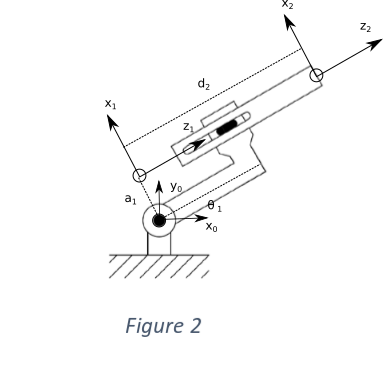
\includegraphics[scale=0.6]{3-4frames.png}
     \end{figure}
     This gives us the DH parameters of
     \begin{center}
     \begin{tabular}{|c|c|c|c|r|}
      \hline
      Link & $\theta_i$ & $d_i$ & $a_i$ & $\alpha_i$ \\
      \hline
      1 & $\theta_1 + \pi/2$ & 0 & $a_1$ & $\pi/2$ \\
      2 & 0 & $d_2$ & 0 & 0 \\
      \hline
     \end{tabular}
     \end{center}
     
     Thus we have
     \[
       A_1(\theta_1) = 
       \begin{bmatrix}
         c_{\theta_1 + \pi/2} & 0 & s_{\theta_1 + \pi/2} & a_1c_{\theta_1 + \pi/2} \\
         s_{\theta_1 + \pi/2} & 0 & -c_{\theta_1 + \pi/2} & a_1s_{\theta_1 + \pi/2} \\
         0 & 1 & 0 & 0 \\
         0 & 0 & 0 & 1
       \end{bmatrix}
     \]
     \[
       A_2(d_2) = 
       \begin{bmatrix}
         1 & 0 & 0 & 0 \\
         0 & 1 & 0 & 0 \\
         0 & 0 & 1 & d_2 \\
         0 & 0 & 0 & 1
       \end{bmatrix}
     \]
     Thus we have that 
     \[
       ^0T_2 = A_1(\theta_1)A_2(d_2)  =
       \begin{bmatrix}
         c_{\theta_1 + \pi/2} & 0 & s_{\theta_1 + \pi/2} & a_1c_{\theta_1 + \pi/2} + d_2s_{\theta_1+\pi/2} \\
         s_{\theta_1 + \pi/2} & 0 & -c_{\theta_1 + \pi/2} & a_1s_{\theta_1 + \pi/2} - d_2c_{\theta_1 + \pi/2}\\
         0 & 1 & 0 & 0 \\
         0 & 0 & 0 & 1
       \end{bmatrix}
     \]
     
     \part 3-6

     I have laid down my coordinate frames as follow

     \begin{figure}[!ht]
      \centering 
      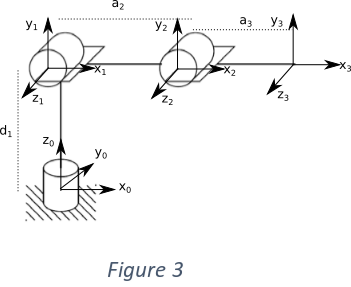
\includegraphics[scale=0.6]{3-6frames.png}
     \end{figure}

     Which gives us the DH parameters of
     \begin{center}
     \begin{tabular}{|c|c|c|c|r|}
      \hline
      Link & $\theta_i$ & $d_i$ & $a_i$ & $\alpha_i$ \\
      \hline
      1 & $\theta_1$ & $d_1$ & 0 & $\pi/2$ \\
      2 & $\theta_2$ & 0 & $a_2$ & 0 \\
      3 & $\theta_3$ & 0 & $a_3$ & 0 \\
      \hline
     \end{tabular}
     \end{center}
     
     Which gives us the following transformations
     \[
       A_1(\theta_1) = 
       \begin{bmatrix}
         c_{\theta_1} & 0 & s_{\theta_1} & 0 \\
         s_{\theta_1} & 0 & -c_{\theta_1} & 0 \\
         0 & 1 & 0 & d_1 \\
         0 & 0 & 0 & 1
       \end{bmatrix}
     \]
     \[
       A_2(\theta_2) = 
       \begin{bmatrix}
         c_{\theta_2} & -s_{\theta_2} & 0 & a_2c_{\theta_2}\\
         s_{\theta_2} & c_{\theta_2} & 0 & a_2s_{\theta_2} \\
         0 & 0 & 1 & 0 \\
         0 & 0 & 0 & 1
       \end{bmatrix}
     \]
     \[
       A_3(\theta_3) = 
       \begin{bmatrix}
         c_{\theta_3} & -s_{\theta_3} & 0 & a_3c_{\theta_3}\\
         s_{\theta_3} & c_{\theta_3} & 0 & a_3s_{\theta_3} \\
         0 & 0 & 1 & 0 \\
         0 & 0 & 0 & 1
       \end{bmatrix}
     \]
     Thus we have that (using the robotics toolbox)
     \[
       ^0T_3 = A_1(\theta_1)A_2(\theta_2)A_3(\theta_3) =
       \begin{bmatrix}
         c_{\theta_2 + \theta_3}c_{\theta_1} & -s_{\theta_2 + \theta_3}c_{\theta_1} & s_{\theta_1} & c_{\theta_1}(a_3c_{\theta_2 + \theta_3} + a_2c_{\theta_2}) \\
         c_{\theta_2 + \theta_3}s_{\theta_1} & -s_{\theta_2 + \theta_3}s_{\theta_1} & -c_{\theta_1} & s_{\theta_1}(a_3c_{\theta_2 + \theta_3} + a_2c_{\theta_2}) \\
         s_{\theta_2 + \theta_3} & c_{\theta_2 + \theta_3} & 0 & d_1 + a_3s_{\theta_2+\theta_3} + a_2s_{\theta_2} \\
         0 & 0 & 0 & 1
       \end{bmatrix}
     \]

     \part 3-6 (new frames)

     I have laid down my coordinate frames as follow

     \begin{figure}[!ht]
      \centering 
      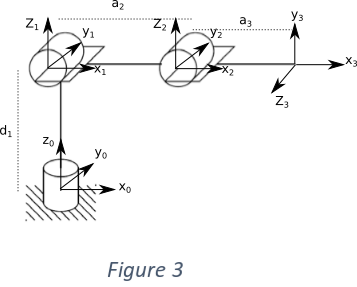
\includegraphics[scale=0.6]{3-6frames2.png}
     \end{figure}
     Thus we have the following transformations
     \[
       A_1(\theta_1) =
       \begin{bmatrix}
         c_{\theta_1} & -s_{\theta_1} & 0 & 0 \\
         s_{\theta_1} & c_{\theta_1} & 0 & 0 \\
         0 & 0 & 1 & d_1 \\
         0 & 0 & 0 & 1
       \end{bmatrix}
     \]
     \[
       A_2(\theta_2) = 
       \begin{bmatrix}
         c_{\theta_2} & 0 & s_{\theta_2} & a_2c_{\theta_2} \\
         0 & 1 & 0 & 0 \\
         -s_{\theta_2} & 0 & c_{\theta_2} & -a_2s_{\theta_2} \\
         0 & 0 & 0 & 1
       \end{bmatrix}
     \]
     \[
       A_3(\theta_3) = 
       \begin{bmatrix}
         c_{\theta_3} & s_{\theta_3} & 0 & a_3c_{\theta_3} \\
         0 & 0 & -1 & 0 \\
         -s_{\theta_3} & c_{\theta_3} & 0 & -a_3s_{\theta_3} \\
         0 & 0 & 0 & 1
       \end{bmatrix}
     \]
     Thus we have that (using matlab)
     \[
       ^0T_3 = A_1(\theta_1)A_2(\theta_2)A_3(\theta_3) =
       \begin{bmatrix}
         c_{\theta_2 + \theta_3}c_{\theta_1} & s_{\theta_2 + \theta_3}c_{\theta_1} & s_{\theta_1} & c_{\theta_1}(a_3c_{\theta_2 + \theta_3} + a_2c_{\theta_2}) \\
         c_{\theta_2 + \theta_3}s_{\theta_1} & -s_{\theta_2 + \theta_3}s_{\theta_1} & -c_{\theta_1} & s_{\theta_1}(a_3c_{\theta_2 + \theta_3} + a_2c_{\theta_2}) \\
         -s_{\theta_2 + \theta_3} & c_{\theta_2 + \theta_3} & 0 & d_1 - a_3s_{\theta_2+\theta_3} - a_2s_{\theta_2} \\
         0 & 0 & 0 & 1
       \end{bmatrix}
     \]
     The representations are different! This is because the axis of rotation for joints 2 and 3 are in the opposite direction compared to the last problem. Besides this they are the same, and dynamically they are the same since there will be a negative sign compared to the DH representation.

     \part
     I have laid down my coordinate frames as follow, (I didn't label the $a_i$ and $d_i$, but it should be fairly obvious from the image).

     \begin{figure}[!ht]
      \centering 
      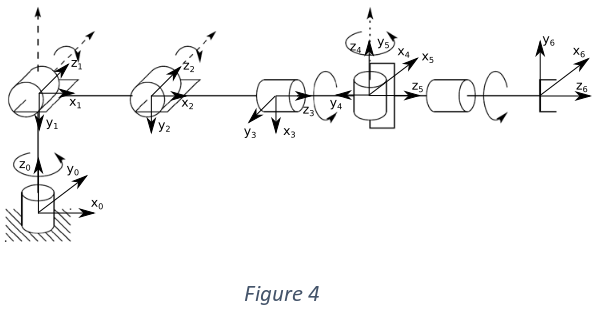
\includegraphics[scale=0.6]{3-8frames.png}
     \end{figure}

     Which gives us the DH parameters of

     \begin{center}
     \begin{tabular}{|c|c|c|c|r|}
      \hline
      Link & $\theta_i$ & $d_i$ & $a_i$ & $\alpha_i$ \\
      \hline
      1 & $\theta_1$ & $d_1$ & 0 & $-\pi/2$ \\
      2 & $\theta_2$ & 0 & $a_2$ & 0 \\
      3 & $\theta_3 + \pi/2$ & 0 & $a_3$ & $\pi/2$ \\
      4 & $\theta_4 + \pi/2$ & $d_1$ & 0 & $\pi/2$ \\
      5 & $\theta_5$ & 0 & 0 & $\pi/2$ \\
      6 & $\theta_6$ & $d_6$ & 0 & 0 \\
      \hline
     \end{tabular}
     \end{center}
     


     
  \end{parts}
\end{problem}

\end{document}
